\documentclass{beamer}
\mode<presentation>
\usepackage{amsmath}
\usepackage{amssymb}
%\usepackage{advdate}
\usepackage{graphicx}
\graphicspath{{../figs/}}
\usepackage{adjustbox}
\usepackage{subcaption}
\usepackage{enumitem}
\usepackage{multicol}
\usepackage{mathtools}
\usepackage{listings}
\usepackage{url}
\def\UrlBreaks{\do\/\do-}
\usetheme{Boadilla}
\usecolortheme{lily}
\setbeamertemplate{footline}
{
  \leavevmode%
  \hbox{%
  \begin{beamercolorbox}[wd=\paperwidth,ht=2.25ex,dp=1ex,right]{author in head/foot}%
    \insertframenumber{} / \inserttotalframenumber\hspace*{2ex} 
  \end{beamercolorbox}}%
  \vskip0pt%
}
\setbeamertemplate{navigation symbols}{}
\let\solution\relax
\usepackage{gvv}
\lstset{
%language=C,
frame=single, 
breaklines=true,
columns=fullflexible
}

\numberwithin{equation}{section}


\title{4.6.8}
\author{EE25BTECH11020 - Darsh Pankaj Gajare}
\begin{document}
\maketitle
% \newpage
% \bigskip
Question:\\
Find the equation of the plane passing through the points $\brak{2,2,-1}$,$\brak{3,4,2}$ and $\brak{7,0,6}$. Also find the equation of the plane passing through $\brak{4,3,1}$ and parallel to the plane obtained above.\\
\solution
\begin{table}[H]
	\centering
	\caption{}
	\begin{tabular}{|c|c|}
\hline
\textbf{Name} & \textbf{Value} \\
\hline
Circle & $\vec{x}^\top\vec{x} - a^2 = 0$ \\
\hline
Line & $\vec{x} = \myvec{\tfrac{a}{\sqrt{2}} \\ 0} + \kappa\myvec{0 \\ 1}$ \\
\hline
\end{tabular}

	\label{}
\end{table}
Let the equation of plane be
\begin{align}
	\vec{n}^\top\vec{x}=C_1
\end{align}
A,B,C satisfies this equation,
\begin{align}
	\vec{n}^\top\vec{A}=C_1,
	\vec{n}^\top\vec{B}=C_1,
	\vec{n}^\top\vec{C}=C_1
\end{align}
\begin{align}
	\myvec{\vec{A}\\\vec{B}\\\vec{C}}^\top\vec{n}=\myvec{C_1\\C_1\\C_1}
\end{align}
Using augmented matrix,
\begin{align}
	\augvec{3}{1}{2&2&-1&C_1\\3&4&2&C_1\\7&0&6&C_1}
\end{align}
$R_1=R_1/2$
\begin{align}
	\augvec{3}{1}{1&1&-0.5&\frac{C_1}{2}\\3&4&2&C_1\\7&0&6&C_1}
\end{align}
$R_2=R_2-3R_1$
\begin{align}
	\augvec{3}{1}{1&1&-0.5&\frac{C_1}{2}\\0&1&3.5&\frac{-C_1}{2}\\7&0&6&C_1}
\end{align}
$R_3=R_3-7R_1$
\begin{align}
	\augvec{3}{1}{1&1&-0.5&\frac{C_1}{2}\\0&1&3.5&\frac{-C_1}{2}\\0&-7&9.5&\frac{-5C_1}{2}}
\end{align}
$R_3=R_3+7R_2$
\begin{align}
	\augvec{3}{1}{1&1&-0.5&\frac{C_1}{2}\\0&1&3.5&\frac{-C_1}{2}\\0&0&34&-6C_1}
\end{align}
\begin{align}
	34z+6C_1=0\implies z=\frac{-3C_1}{17} 
\end{align}
\begin{align}
	y+3.5z+0.5C_1=0\implies y=\frac{2C_1}{17}
\end{align}
\begin{align}
	\augvec{3}{1}{1&1&-0.5&\frac{C_1}{2}\\0&1&3.5&\frac{-C_1}{2}\\0&-7&9.5&\frac{-5C_1}{2}}
\end{align}
\begin{align}
	x+y-0.5z=0.5C_1\implies x=\frac{5C_1}{17}
\end{align}
Let $C_1=17$
\begin{align}
	\vec{n}=\myvec{5\\2\\-3},C_1=17
\end{align}
Equation of plane parallel to given plane passing through D,
\begin{align}
	\vec{n}^\top\vec{x}=C_2
\end{align}
\begin{align}
	\vec{n}^\top\vec{D}=C_2
\end{align}
\begin{align}
	C_2=\myvec{5&2&-3}\myvec{4\\3\\1}
\end{align}
\begin{align}
	C_2=23
\end{align}
Equation of plane
\begin{align}
	\myvec{5\\2\\-3}^\top\vec{x}=23
\end{align}

\begin{figure}[H]
	\centering
	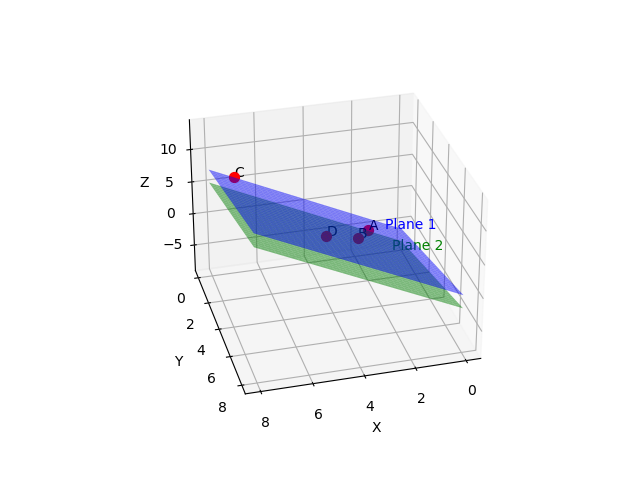
\includegraphics[scale=0.5]{img1}
	\caption*{}
	\label{img1}
\end{figure}
Plot using Python:
\begin{figure}[H]
	\centering
	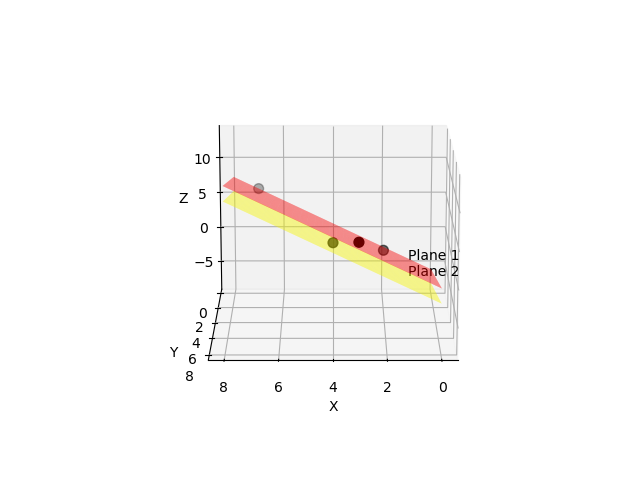
\includegraphics[scale=0.5]{img2}
	\caption*{}
	\label{img2}
\end{figure}
\end{document}

